\documentclass[11pt,a4paper]{article}
\usepackage[utf8]{inputenc}
\usepackage[vietnamese]{babel}
\usepackage{amsmath,amssymb}
\usepackage[version=4]{mhchem}
\usepackage{geometry}
\geometry{top=1.5cm,bottom=1.2cm,left=1.4cm,right=1.4cm,headheight=28pt,headsep=12pt,footskip=18pt}
\usepackage{graphicx}
\usepackage{xcolor}
\usepackage{tabularx}
\usepackage{array}
\usepackage{tikz}
\usepackage{fancyhdr}
\usepackage{enumitem}

\definecolor{hfRed}{HTML}{D32F2F}
\definecolor{hfGreen}{HTML}{8BC390}
\definecolor{mainGreen}{HTML}{2E7D32}

\usepackage{ex_test}

\pagestyle{fancy}
\fancyhf{}
\renewcommand{\headrulewidth}{0.75pt}
\renewcommand{\headrule}{\hbox to\headwidth{\color{hfGreen}\leaders\hrule height \headrulewidth\hfill}}
\renewcommand{\footrulewidth}{0.75pt}
\renewcommand{\footrule}{\hbox to\headwidth{\color{hfGreen}\leaders\hrule height \footrulewidth\hfill}}

\fancyhead[L]{\small\itshape\color{hfRed}Tài liệu lưu hành nội bộ}
\fancyhead[R]{\small\color{hfRed}Thầy \textbf{TRẦN VĂN THẠNH} - 0777.470.803}

\fancyfoot[L]{\footnotesize\itshape\color{hfRed}CS1: 6/15 Nguyễn Hoàng, P. Kim Long, TP Huế \quad|\quad CS2: 24 Đặng Thái Thân, TP Huế}
\fancyfoot[R]{\small\textbf{\color{hfRed}Trang \thepage}}

\setlength{\parindent}{0pt}
\setlength{\parskip}{1.5pt}

\begin{document}

\begin{minipage}[t]{0.45\textwidth}
\textbf{SỞ GD\&ĐT BẮC NINH}\\
\textbf{CỤM TRƯỜNG THPT BẮC NINH}\\
\textit{ĐỀ CHÍNH THỨC}\\
\textit{(Đề thi có 04 trang)}
\end{minipage}
\hfill
\begin{minipage}[t]{0.52\textwidth}
\raggedleft
\textbf{\color{hfRed}HƯỚNG TỚI KÌ THI TỐT NGHIỆP THPT}\\
\textbf{MÔN: HOÁ HỌC -- KHỐI 12}\\
\textit{Thời gian làm bài: 50 phút (không kể thời gian phát đề)}\\
\textbf{MÃ ĐỀ THI: 101}
\end{minipage}

\vspace{3pt}
\noindent
\textit{Họ, tên thí sinh:} \dotfill \textit{Lớp:} \dotfill \textit{SBD:} \dotfill

\vspace{2pt}
\noindent
\textit{\footnotesize (Cho biết nguyên tử khối: H = 1; C = 12; N = 14; O = 16; P = 31; Cl = 35,5; K = 39; Fe = 56; Ag = 108).}

\vspace{2pt}
\noindent
\textbf{\color{mainGreen}PHẦN I (4,5 điểm -- 18 câu): Câu trắc nghiệm nhiều phương án lựa chọn.}\\
\textit{Thí sinh trả lời từ câu 1 đến câu 18. Mỗi câu hỏi thí sinh chỉ chọn một phương án.}

\Opensolutionfile{ans}[ans-bn-hs]

\begin{ex}
Các đồng vị của cùng một nguyên tố hoá học là những nguyên tử có cùng số proton nhưng khác nhau ...(1).... Nội dung phù hợp trong chỗ trống (1) là:
\choice
{số electron.}
{điện tích hạt nhân.}
{\True số neutron.}
{số hiệu nguyên tử.}

\end{ex}

\begin{ex}
Dụng cụ trong hình bên dưới có tên gọi là gì?
\begin{center}
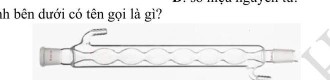
\includegraphics[width=6.5cm]{images_bacninh_2025/cau2_ong_sinh_han.png}
\end{center}
\choice
{Pipette.}
{\True Ống sinh hàn.}
{Ống đong.}
{Burette.}

\end{ex}

\begin{ex}
Cho cấu hình electron nguyên tử của các nguyên tố: X: $1s^2 2s^2 2p^6$; Y: $1s^2 2s^2 2p^6 3s^2$; Z: $1s^2 2s^2 2p^3$; T: $1s^2 2s^2 2p^6 3s^2 3p^5$. Nhận xét nào sau đây đúng?
\choice
{X là khí hiếm, Z là kim loại.}
{Tất cả các nguyên tố trên đều thuộc cùng một chu kì trong bảng tuần hoàn.}
{Trong 4 nguyên tố trên, chỉ có Z là phi kim.}
{\True Liên kết trong hợp chất tạo bởi Y và T là liên kết ion.}

\end{ex}

\begin{ex}
Trong máu người trưởng thành, khỏe mạnh vào lúc đói có một lượng nhỏ glucose với nồng độ khoảng 4,4 – 7,2 mmol/L (hay 80 – 130 mg/dL). Công thức cấu tạo dạng mạch hở của glucose là
\choice
{\True \ce{CH2OH[CHOH]4CHO}.}
{\ce{CH2OH[CHOH]5CHO}.}
{\ce{CH2OH[CHOH]4CH2OH}.}
{\ce{CH2OH[CHOH]4COOH}.}

\end{ex}

\begin{ex}
Liên kết $\sigma$ là liên kết được hình thành do
\choice
{lực hút tĩnh điện giữa hai ion.}
{sự xen phủ bên của 2 orbital.}
{\True sự xen phủ trục của hai orbital.}
{sự nhường và nhận electron giữa 2 nguyên tử.}

\end{ex}

\begin{ex}
Cho phản ứng: $2\ce{SO2}(g) + \ce{O2}(g) \rightleftharpoons 2\ce{SO3}(g)$, $\Delta H < 0$. Yếu tố nào sau đây không làm chuyển dịch cân bằng của phản ứng trên?
\choice
{Áp suất chung của hệ.}
{\True Chất xúc tác.}
{Nồng độ các chất phản ứng.}
{Nhiệt độ của hệ.}

\end{ex}

\begin{ex}
Amine nào sau đây là amine bậc hai?
\choice
{Methylamine.}
{\True Dimethylamine.}
{Ethylamine.}
{Trimethylamine.}

\end{ex}

\begin{ex}
Thuỷ phân hoàn toàn saccharose ($\ce{C12H22O11}$) trong môi trường acid, thu được sản phẩm nào?
\choice
{\True Glucose và fructose.}
{Chỉ có fructose.}
{Chỉ có glucose.}
{Glucose và maltose.}

\end{ex}

\begin{ex}
Nhỏ vài giọt nước bromine vào ống nghiệm chứa aniline, hiện tượng quan sát được là
\choice
{\True có kết tủa màu trắng.}
{có bọt khí thoát ra.}
{xuất hiện màu xanh.}
{xuất hiện màu tím.}

\end{ex}

\begin{ex}
Để phân biệt ba bình khí không màu, mất nhãn: propane, ethylene và acetylene, người ta có thể dùng lần lượt các thuốc thử nào sau đây?
\choice
{\True Dung dịch $\ce{AgNO3/NH3}$ và dung dịch $\ce{Br2}$.}
{Dung dịch $\ce{KMnO4}$ và dung dịch $\ce{NaOH}$.}
{Dung dịch $\ce{Br2}$ và que đóm cháy dở.}
{Quỳ tím ẩm và dung dịch $\ce{Br2}$.}

\end{ex}

\begin{ex}
Acid béo omega-3 và omega-6 là các acid béo không no với liên kết đôi đầu tiên ở vị trí số 3 và 6 khi đánh số từ nhóm methyl, chúng đều có vai trò quan trọng đối với cơ thể, giúp phòng ngừa nhiều loại bệnh. Chất nào sau đây thuộc loại acid béo omega-3?
\begin{center}
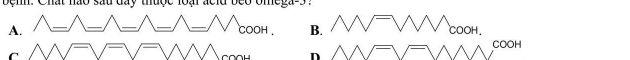
\includegraphics[width=13.5cm]{images_bacninh_2025/cau11_acid_beo.png}
\end{center}
\choice
{\True Chất A.}
{Chất B.}
{Chất C.}
{Chất D.}

\end{ex}

\begin{ex}
Isoamyl acetate là một ester có mùi thơm dễ chịu của chuối chín, được dùng làm hương liệu thực phẩm. Công thức cấu tạo thu gọn của isoamyl acetate là
\choice
{\ce{HCOOCH2CH2CH(CH3)2}.}
{\True \ce{CH3COOCH2CH2CH(CH3)2}.}
{\ce{CH3COOCH(CH3)CH2CH3}.}
{\ce{CH3COOCH2CH(CH3)2}.}

\end{ex}

\begin{ex}
Sodium lauryl sulfate là một trong những chất giặt rửa tổng hợp phổ biến có công thức cấu tạo như sau:
\begin{center}
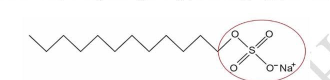
\includegraphics[width=7cm]{images_bacninh_2025/cau13_sls.png}
\end{center}
Đặc điểm của nhóm được khoanh tròn trong công thức trên là gì?
\choice
{Tạo kết tủa với nước cứng.}
{Không phân cực.}
{Kị nước.}
{\True Ưa nước.}

\end{ex}

\begin{ex}
Để khảo sát ảnh hưởng của cấu tạo gốc hydrocarbon đến lực base của các amine no, đơn chức, mạch không nhánh, một nhóm học sinh tiến hành đo pH của các dung dịch amine gồm: methylamine, ethylamine và propylamine. Trong kế hoạch thí nghiệm, nhóm đã liệt kê các yếu tố sau:\\
(1) Nồng độ mol của các dung dịch amine.\\
(2) Nhiệt độ của các dung dịch khi đo pH.\\
(3) Loại amine được sử dụng trong mỗi mẫu đo.\\
(4) Thể tích dung dịch amine lấy ra để đo pH.\\
Những yếu tố nào cần được thiết lập giống nhau ở tất cả các mẫu thử?
\choice
{(1), (2), (3).}
{(1), (3), (4).}
{(2), (3), (4).}
{\True (1), (2), (4).}

\end{ex}

\begin{ex}
Chất nào sau đây thuộc loại hợp chất alcohol?
\choice
{\True \ce{C3H5(OH)3}.}
{\ce{CH3COOH}.}
{\ce{H-CHO}.}
{\ce{CH3-CO-CH3}.}

\end{ex}

\begin{ex}
Chất X có màu trắng, dạng sợi, không mùi vị, không tan trong nước, là thành phần chính tạo nên màng tế bào thực vật. Chất X là
\choice
{saccharose.}
{\True cellulose.}
{tinh bột.}
{glucose.}

\end{ex}

\begin{ex}
Ở điều kiện thường, thực hiện thí nghiệm với khí $\ce{NH3}$ như sau:\\
Bước 1. Nạp đầy khí $\ce{NH3}$ vào bình thủy tinh rồi đậy bình bằng nút cao su.\\
Bước 2. Dùng ống thủy tinh vuốt nhọn đầu nhúng vào nước, xuyên ống thủy tinh qua nút cao su rồi lắp bình thủy tinh lên giá như hình vẽ bên.
\begin{center}
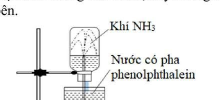
\includegraphics[width=4.5cm]{images_bacninh_2025/cau17_dai_phun_nuoc.png}
\end{center}
Phát biểu nào sau đây là không đúng?
\choice
{Trong phản ứng $\ce{NH3 + H2O <=> NH4+ + OH-}$. Theo thuyết Brønsted – Lowry, $\ce{NH3}$ đóng vai trò là base.}
{Thí nghiệm trên chứng minh khí $\ce{NH3}$ tan tốt trong nước.}
{\True Tia nước phun mạnh vào bình do áp suất trong bình cao hơn áp suất không khí.}
{Dung dịch $\ce{NH3}$ có môi trường base.}

\end{ex}

\begin{ex}
Cho phản ứng tổng hợp ammonia: $\ce{N2}(g) + 3\ce{H2}(g) \rightleftharpoons 2\ce{NH3}(g)$. Cho năng lượng liên kết $E_b$ ở điều kiện chuẩn: $E_b(\ce{N\equiv N}) = 945\text{ kJ/mol}$; $E_b(\ce{H-H}) = 436\text{ kJ/mol}$; $E_b(\ce{N-H}) = 386\text{ kJ/mol}$. Biến thiên enthalpy chuẩn ($\Delta_r H^\circ_{298}$) của phản ứng là:
\choice
{-935 kJ.}
{-92 kJ.}
{1095 kJ.}
{\True -63 kJ.}

\end{ex}

\Closesolutionfile{ans}

\vspace{6pt}
\noindent
\textbf{\color{mainGreen}PHẦN II (4,0 điểm -- 4 câu): Câu trắc nghiệm đúng sai.}\\
\textit{Thí sinh trả lời từ câu 1 đến câu 4. Trong mỗi ý a), b), c), d) ở mỗi câu, thí sinh chọn đúng hoặc sai.}

\setcounter{ex}{0}

\begin{ex}
Cellulose là thành phần chính của thành tế bào thực vật, làm nên bộ khung của cây cối. Cellulose có nhiều trong bông, đay, tre, nứa, gỗ,... Từ cellulose người ta điều chế được cellulose acetate (có thành phần chủ yếu là cellulose triacetate và cellulose diacetate) theo các phương trình sau:\\
(1) $[\ce{C6H7O2(OH)3}]_n + 2n(\ce{CH3CO})_2\ce{O} \rightarrow [\ce{C6H7O2(OCOCH3)2(OH)}]_n + 2n\ce{CH3COOH}$.\\
(2) $[\ce{C6H7O2(OH)3}]_n + 3n(\ce{CH3CO})_2\ce{O} \rightarrow [\ce{C6H7O2(OCOCH3)3}]_n + 3n\ce{CH3COOH}$.
\choiceTF
{Trong mỗi phân tử cellulose có 3 nhóm hydroxy nên cellulose có khả năng phản ứng với $\ce{Cu(OH)2}$ trong môi trường kiềm ở nhiệt độ thường tạo dung dịch màu xanh lam.}
{Phân tử khối của cellulose là 162.}
{\True Cellulose là nguyên liệu trong sản xuất ethanol và thuốc súng không khói.}
{Khi phân tích thành phần nguyên tố của một mẫu cellulose acetate người ta thu được phần trăm khối lượng carbon là 49,875\%. Vậy thành phần phần trăm khối lượng oxygen trong cellulose acetate trên là 34,64\%. Giả sử trong cellulose acetate chỉ có cellulose triacetate và cellulose diacetate. \textit{(kết quả làm tròn đến hàng phần trăm)}.}

\end{ex}

\begin{ex}
Cho các phát biểu sau:
\choiceTF
{\True Trong không khí, $\ce{N2}$ chiếm khoảng 78\% về thể tích.}
{Trong phản ứng giữa $\ce{N2}$ và $\ce{H2}$ thì $\ce{N2}$ vừa là chất oxi hóa, vừa là chất khử.}
{Khi điều chế khí nitrogen, cách thu khí ở hình 1 là phù hợp nhất.}
{\True Phần lớn $\ce{N2}$ được sử dụng để tổng hợp $\ce{NH3}$ từ đó sản xuất nitric acid, phân bón, ...}
\begin{center}
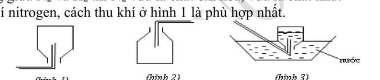
\includegraphics[width=9cm]{images_bacninh_2025/p2_cau2_thu_khi.png}
\end{center}

\end{ex}

\begin{ex}
Aspirin (hay acetylsalicylic acid), là một dẫn xuất của salicylic acid được sử dụng để hạ sốt và giảm đau nhẹ đến trung bình do tình trạng đau nhức cơ, răng, cảm lạnh đau đầu và sưng tấy do viêm khớp. Một nhóm học sinh thực hiện tổng hợp Aspirin trong phòng thí nghiệm như sau:\\
Bước 1: Cho 75,0 gam salicylic acid khan và 105,0 mL acetic anhydride ($d = 1{,}08\text{ g/mL}$) vào bình cầu 250 mL; thêm 4,0 mL sulfuric acid đặc vào và lắc kỹ. Sau đó, khuấy khối phản ứng ở 50–60°C trong khoảng 45 phút cho đến khi tan hết phần chất rắn.\\
Bước 2: Dùng nước đá để làm lạnh hỗn hợp phản ứng đến nhiệt độ nhỏ hơn 10°C. Cho hỗn hợp vào cốc lớn, thêm từ từ 750 mL nước cất và khuấy kỹ, aspirin sẽ kết tủa. Lọc lấy sản phẩm bằng phễu lọc Buchner.\\
Bước 3: Hòa tan aspirin thô trong 100 mL ethanol 90°, đun nóng để tan hoàn toàn, sau đó đổ dung dịch này từ từ vào 450 mL nước nóng khoảng 50°C, đun nóng nhẹ cho chất rắn tan hết. Để nguội dung dịch thu được đến nhiệt độ phòng. Aspirin kết tinh dưới dạng tinh thể, lọc và hút hết nước, sấy khô ở 50°C.\\
Bước 4: Cân sản phẩm thu được 83,1 gam aspirin. Hiệu suất của quá trình là $x$\%.\\
Biết phương trình hóa học điều chế aspirin từ salicylic acid được biểu diễn như sau:
\begin{center}
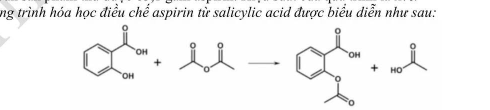
\includegraphics[width=10.5cm]{images_bacninh_2025/p2_cau3_aspirin.png}
\end{center}
\choiceTF
{\True Giá trị của $x$ là 85\% \textit{(kết quả làm tròn đến hàng đơn vị)}.}
{Aspirin tan trong nước nhiều hơn salicylic acid.}
{Aspirin là hợp chất hữu cơ tạp chức, trong đó có chức ester và chức phenol.}
{\True Phương pháp tách và tinh chế aspirin ở trên là phương pháp kết tinh.}

\end{ex}

\begin{ex}
Trong quản lý chất lượng dầu mỡ công nghiệp và thực phẩm, chỉ số acid được định nghĩa là số miligam KOH cần dùng để trung hòa hết lượng acid béo tự do có trong 1,00 gam chất béo; chỉ số xà phòng hóa là số miligam KOH cần dùng để xà phòng hóa hoàn toàn các triglyceride và trung hòa hết lượng acid béo tự do có trong 1,00 gam chất béo. Để kiểm định một lô dầu cọ tinh luyện (mẫu X) gồm các triglyceride và một lượng nhỏ acid béo tự do (giả thiết các gốc hydrocarbon mạch dài trong X chỉ gồm palmitate – $\ce{C15H31}$, stearate – $\ce{C17H35}$ và oleate – $\ce{C17H33}$), phòng thí nghiệm tiến hành ba thí nghiệm độc lập sau:\\
- Thí nghiệm 1: Hòa tan 10,00 gam mẫu X vào hỗn hợp dung môi trung tính (ethanol – ether) rồi tiến hành chuẩn độ bằng dung dịch chuẩn KOH 0,10 M. Đến điểm kết thúc chuẩn độ, thể tích dung dịch KOH đã tiêu tốn là 4,50 mL.\\
- Thí nghiệm 2: Đun nóng 50,00 gam mẫu X với 150,00 mL dung dịch KOH 1,50 M trong cồn đến khi phản ứng xà phòng hóa xảy ra hoàn toàn. Để trung hòa lượng KOH còn dư sau phản ứng cần vừa đủ 51,00 mL dung dịch chuẩn HCl 1,00 M.\\
- Thí nghiệm 3: Tiến hành phản ứng hydrogen hóa hoàn toàn 50,00 gam mẫu X (xúc tác Ni, $t^\circ, p$), thấy thể tích khí $\ce{H2}$ phản ứng tối đa là 1,2395 lít (đkc).\\
Cho các phát biểu sau:
\choiceTF
{Ở Thí nghiệm 3, phản ứng hydrogen hóa làm tăng số liên kết pi trong phân tử các triglyceride, từ đó giúp dầu cọ chuyển từ dạng lỏng sang dạng rắn và hạn chế bị ôi thiu.}
{\True Trong Thí nghiệm 1, dung môi được sử dụng là hỗn hợp ethanol – ether với mục đích hòa tan hoàn toàn mẫu dầu mà không làm thay đổi lượng acid béo tự do cần chuẩn độ.}
{\True Chỉ số xà phòng hóa của mẫu dầu cọ X luôn có giá trị lớn hơn chỉ số acid của nó.}
{\True Từ các số liệu thực nghiệm, xác định được chỉ số acid và chỉ số xà phòng hóa của mẫu dầu cọ X lần lượt là 2,52 và 194,88.}

\end{ex}

\vspace{6pt}
\noindent
\textbf{\color{mainGreen}PHẦN III (1,5 điểm -- 6 câu): Câu trắc nghiệm yêu cầu trả lời ngắn.}\\
\textit{Thí sinh trả lời từ câu 1 đến câu 6.}

\setcounter{ex}{0}

\begin{ex}
Cho các phát biểu sau:\\
(a) Phân tử methyl methacrylate có một liên kết pi trong phân tử.\\
(b) Cho dung dịch methylamine vào ống nghiệm đựng dung dịch iron(III) chloride thấy xuất hiện kết tủa nâu đỏ.\\
(c) Methylamine làm quỳ tím ẩm hóa xanh.\\
(d) Glucose và maltose đều có nhóm -OH hemiacetal.\\
(e) Dung dịch Fructose và dung dịch saccharose đều hòa tan được $\ce{Cu(OH)2}$, tạo thành dung dịch ở điều kiện thường.\\
Có bao nhiêu phát biểu đúng?
\newline\textbf{Trả lời:} \dotfill
\end{ex}

\begin{ex}
Xăng sinh học E5 (chứa 5\% ethanol về thể tích, còn lại là xăng, giả thiết chỉ là octane). Khi được đốt cháy hoàn toàn, 1 mol ethanol tỏa ra lượng nhiệt là 1365,0 kJ và 1 mol isooctane ($\ce{C8H18}$) tỏa ra lượng nhiệt là 5928,7 kJ. Trung bình, một chiếc xe máy di chuyển được 1 km thì cần một nhiệt lượng chuyển thành công cơ học có độ lớn là 212 kJ. Để đi được quãng đường 100 km cần dùng bao nhiêu lít xăng E5? \textit{(Không làm tròn kết quả các phép tính trung gian, chỉ làm tròn kết quả cuối cùng đến hàng phần trăm)}. Biết rằng, hiệu suất sử dụng nhiên liệu của động cơ là 25\%, khối lượng riêng của ethanol là 0,8 g/mL, của isooctane là 0,7 g/mL.
\newline\textbf{Trả lời:} \dotfill
\end{ex}

\begin{ex}
Cho phương trình hóa học của các phản ứng được đánh số thứ tự từ 1 tới 6 dưới đây:\\
(1) $6n\ce{CO2} + 5n\ce{H2O} \xrightarrow{\text{chlorophyll}} (\ce{C6H10O5})_n + 6n\ce{O2}$.\\
(2) $\ce{C6H12O6} \text{ (glucose)} \xrightarrow{\text{enzyme}} 2\ce{CH3-CHOH-COOH} \text{ (lactic acid)}$.\\
(3) $(\ce{C6H10O5})_n \text{ (tinh bột)} + n\ce{H2O} \xrightarrow{\ce{H^+}, t^\circ} n\ce{C6H12O6} \text{ (glucose)}$.\\
(4) $\ce{C6H12O6} \text{ (glucose)} \xrightarrow{\text{enzyme}} 2\ce{C2H5OH} + 2\ce{CO2}$.\\
(5) $(\ce{C17H35COO})_3\ce{C3H5} + 3\ce{NaOH} \xrightarrow{t^\circ} 3\ce{C17H35COONa} + \ce{C3H5(OH)3}$.\\
(6) $\ce{C6H12O6} + 2[\ce{Ag(NH3)2}]\ce{OH} \xrightarrow{t^\circ} \ce{CH2OH(CHOH)4COONH4} + 2\ce{Ag} + 3\ce{NH3} + \ce{H2O}$.\\
Gán số thứ tự phương trình hoá học của các phản ứng theo tên gọi: xà phòng hóa, quang hợp, lên men rượu, tráng gương và sắp xếp theo trình tự thành dãy bốn số (Ví dụ: 1234, 4321,...)
\newline\textbf{Trả lời:} \dotfill
\end{ex}

\begin{ex}
Phân bón NPK hỗn hợp được sản xuất từ các muối gồm: diammonium phosphate ($(\ce{NH4})_2\ce{HPO4}$), ammonium nitrate ($\ce{NH4NO3}$), potassium chloride ($\ce{KCl}$), cùng một lượng nhỏ tạp chất và chất độn không chứa các nguyên tố N, P, K. Thành phần dinh dưỡng quy đổi về \% khối lượng các chất/nguyên tố trong một loại phân bón NPK được cho trong bảng sau:
\begin{center}
\begin{tabular}{|c|c|c|c|}
\hline
\textbf{Thành phần quy đổi} & \textbf{N} & \textbf{$\ce{P2O5}$} & \textbf{$\ce{K2O}$} \\
\hline
\textbf{\% khối lượng} & 17,00\% & 14,20\% & 18,80\% \\
\hline
\end{tabular}
\end{center}
Phần trăm theo khối lượng của hợp chất ammonium nitrate ($\ce{NH4NO3}$) trong loại phân bón NPK trên là $x$\%. Xác định giá trị của $x$ \textit{(không làm tròn kết quả các phép tính trung gian, chỉ làm tròn kết quả cuối cùng đến hàng phần mười)}.
\newline\textbf{Trả lời:} \dotfill
\end{ex}

\begin{ex}
Cho các chất sau: triolein, saccharose, amylopectin, methyl acetate, fructose, cellulose. Có bao nhiêu chất bị thủy phân trong môi trường acid?
\newline\textbf{Trả lời:} \dotfill
\end{ex}

\begin{ex}
Theo Tiêu chuẩn Việt Nam TCVN 7624 : 2007, khi chế tạo gương, chiều dày lớp bạc phủ trên bề mặt tấm kính (quy ra tổng lượng bạc trên một đơn vị $\text{m}^2$ kính) phải đạt tối thiểu $0{,}7\text{ g}\cdot\text{m}^{-2}$. Một công ty cần sản xuất $18000\text{ m}^2$ gương có độ dày lớp bạc phủ ở mức $0{,}72\text{ g}\cdot\text{m}^{-2}$. Để tạo ra bạc, người ta tiến hành theo sơ đồ phản ứng như sau:
\begin{center}
$\text{Saccharose} \xrightarrow{+\ce{H2O}, \ce{H^+}, t^\circ} \text{Dung dịch X} \xrightarrow{\text{trung hòa acid}} \text{Dung dịch Y} \xrightarrow{+[\ce{Ag(NH3)2}]\ce{OH}, t^\circ} \ce{Ag}$.
\end{center}
Biết hiệu suất cả quá trình là 80\%. Để sản xuất lượng gương với độ phủ bạc như trên, công ty đó cần sử dụng lượng saccharose ít nhất là bao nhiêu kg? \textit{(kết quả làm tròn đến chữ số phần chục, chỉ làm tròn ở phép tính cuối)}.
\newline\textbf{Trả lời:} \dotfill
\end{ex}

\vspace{10pt}
\begin{center}
\textbf{-------------------------- HẾT --------------------------}
\end{center}

\end{document}
